\chapter{Měření elektrického výkonu}

Správnost odvozeného a identifikovaného modelu robota je potřeba ověřit a porovnat se skutečným měřením elektrického výkonu. Měření výkonu bylo provedeno podle schématu na obrázku \ref{mereni_vykonu_pic}. Měřicí sestava je připojena na svorky napájecího vedení mezi elektrickou zásuvkou a skříní s řídicím systémem a napájením robota. Sestava je tvořena měřicí kartou WAGO-I/O-SYSTEM 750 připojenou k průmyslovému PLC Siemens S7-300 CPU 315-2PN/DP. Měřicí karta WAGO obsahuje svorky pro měření napětí a proudu v třífázové síti. 

\begin{figure}[ht]
\includegraphics[width=0.9\textwidth]{mereni_vykonu_obr}
\caption{Schéma zapojení soustavy pro měření výkonu.}
\label{mereni_vykonu_pic}
\end{figure}

Pro účely měření výkonu robotu KUKA KR5 Arc byla karta nakonfigurována pro měření činného výkonu na každé jednotlivé fázi zvlášť. Výsledný celkový výkon je poté podle vzorce \ref{3ph_power_eq} roven součtu výkonů všech jednotlivých fází. Měření výkonu je prováděno s přesností na desetiny wattu. Vzorkovací perioda měření je 40 ms. 

\section{Měřicí karta WAGO-I/O-SYSTEM 750}

Měřicí karta WAGO-I/O-SYSTEM 750 [\cite{wago}] je určena pro měření elektrických veličin v třífázové síti. Je navržena pro použití v průmyslovém prostředí v kombinaci s průmyslovým počítačem PLC. 

Karta je opatřena svorkami pro měření napětí a proudu na každé fázi zvlášť. Měření proudu je prováděno pomocí proudového transformátoru převádějícího měřený proud na napětí. 

Kartu je možné nakonfigurovat pro současné měření až čtyř elektrických veličin jako je stejnosměrné (DC) a střídané (AC) napětí, proud, výkon, frekvence, fázový posuv a další, a to pro každou fázi zvlášť. Navíc je karta schopna provádět analýzu harmonických složek signálu pro vybranou fázi a to až pro 3 vybrané harmonické složky z rozsahu 1. a 41. harmonické. 

\begin{figure}[ht]
    \includegraphics[width=0.3\textwidth]{wago_obr}
    \caption{Měřicí karta WAGO-I/O-SYSTEM 750.}
    \label{wago_pic}
\end{figure}

Změřené veličiny posílá karta přímo na vstupy připojeného PLC, které je dále zpracovává. Měřicí karta se vstupními svorkami je na obrázku \ref{wago_pic}. Technické parametry a podrobnější informace o použití karty je možné nalézt v jejím manuálu [\cite{wago}].

\section{PLC Siemens S7-300}

Průmyslové PLC Siemens S7-300 CPU 315-2PN/DP [\cite{siemens_plc}] zpracovává změřená data, která jsou posílána kartou WAGO 750. PLC tato data cyklicky čte ze vstupů a převádí je do 32-bitového hexadecimálního tvaru. Následně jsou 32-bitová data rozdělena na horních a spodních 16 bitů a opatřena identifikátory. 

Všechna přečtená data s příslušnými identifikátory jsou poté spojena do jedné zprávy, která je navíc ještě opatřena časovou známkou udávající čas o tom, kdy byla data vytvořena. Celá zpráva je nakonec odeslána jako jeden paket pomocí protokolu UDP v síti Profinet.  

Kompletní program pro sběr měřených dat a jejich odesílání v síti Profinet byl vytvořen Ing. Vojtěchem Pavlíkem v rámci jeho diplomové práce [\cite{vojtech_pavlik}]. 

Programování a konfigurace PLC je prováděna pomocí nástroje TIA Portal společnosti SIEMENS. Podrobné informace k PLC S7-300 jsou k dispozici v jeho dokumentaci [\cite{siemens_plc}].  

\section{Aplikace DEPO} 
\label{aplikacedepo}
Za účelem ukládání změřených dat byla panem Ondřejem Fialou vytvořena aplikace DEPO. Aplikace je napsaná ve skriptovací programovacím jazyce RUBY. Spouští se pomocí příkazového řádku na osobním počítači připojeném k Ethernetové síti, ke které je připojeno i měřicí PLC. 

Aplikace přijímá data odesílaná měřicím PLC přes protokol UDP. Přijatá data se poté ukládají jako dokument do databáze MongoDB, ke které je počítač připojený. Uložená data v databázi je poté možné exportovat a následně analyzovat.

Pro správnou funkci aplikace je nutné správně nastavit adresu IP měřícího PLC a číslo portu, na kterém má aplikace odesílaná data číst. Nastavení funkčnosti aplikace DEPO se provádí pomocí konfiguračního souboru. Ten obsahuje informace o IP adrese a portu na kterém má data přijímat a dále adresu, název a kolekci databáze, do které se mají data ukládat.

Protože je aplikace napsaná ve interpretovaném skriptovacím jazyce RUBY, je možné jí spouštět na libovolném operačním systému, který podporuje spouštění RUBY skriptů. 
